\chapter{Theoretische Achtergrond}
\label{hst-theorie}
Dit hoofdstuk bevat de theoretische concepten die nodig zijn om de gebruikte aanpak zo goed mogelijk te begrijpen. Het bevat een beschrijving van de gebruikte neurale netwerken en van een aantal concepten uit de statistiek.

\section{Neurale Netwerken}
Deze sectie geeft een inleiding tot de gebruikte neurale netwerken. Een eerste deel handelt over het eenvoudigste type neuraal netwerk (feed forward), dat de basis vormt voor de varianten die wij gebruiken. Daarna lichten we enkele meer complexe netwerken toe: recurrente en convolutionele neurale netwerken, alsook Long Short Term Memory netwerken. 

\subsection{Feed Forward Neurale Netwerken}
Om een feed forward neuraal netwerk te begrijpen is het concept perceptron nodig. \todo{perceptron nog uitleggen}
\paragraph{Concept} % (fold)
\label{par:concept}
Een feed forward neural netwerk is een van de eenvoudigste neurale netwerken. Het bestaat uit een input laag, een aantal verborgen lagen en een output laag. De outputs van elke laag worden enkel doorgegeven aan de volgende laag, er zijn dus geen cycli in het netwerk (zie figuur \ref{fig:ffnn}. De output kan indien nodig nog door een activatiefunctie worden veranderd.\cite{Bishop:1995:NNP:525960}

\begin{figure}
\def\layersep{2.5cm}
\centering
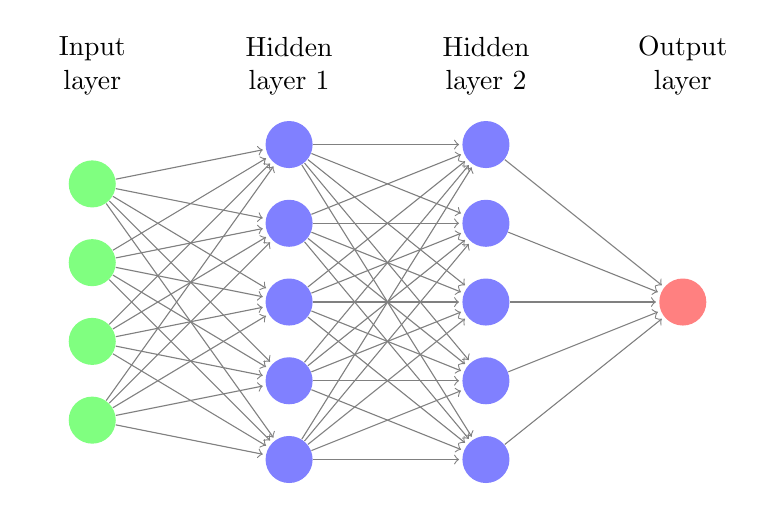
\begin{tikzpicture}[shorten >=1pt,->,draw=black!50, node distance=\layersep]
    \tikzstyle{every pin edge}=[<-,shorten <=1pt]
    \tikzstyle{neuron}=[circle,fill=black!25,minimum size=17pt,inner sep=0pt]
    \tikzstyle{input neuron}=[neuron, fill=green!50];
    \tikzstyle{output neuron}=[neuron, fill=red!50];
    \tikzstyle{hidden neuron}=[neuron, fill=blue!50];
    \tikzstyle{annot} = [text width=4em, text centered]

    % Draw the input layer nodes
    \foreach \name / \y in {1,...,4}
    % This is the same as writing \foreach \name / \y in {1/1,2/2,3/3,4/4}
        \node[input neuron] (I-\name) at (0,-\y) {};

    % Draw the hidden layer nodes
    \foreach \name / \y in {1,...,5}
        \path[yshift=0.5cm]
            node[hidden neuron] (H1-\name) at (\layersep,-\y cm) {};

    % Draw the hidden layer nodes
    \foreach \name / \y in {1,...,5}
        \path[yshift=0.5cm]
            node[hidden neuron] (H2-\name) at (2*\layersep,-\y cm) {};

    % Draw the output layer node
    \node[output neuron, right of=H2-3] (O) {};

    % Connect every node in the input layer with every node in the
    % hidden layer.
    \foreach \source in {1,...,4}
        \foreach \dest in {1,...,5}
            \path (I-\source) edge (H1-\dest);

    \foreach \source in {1,...,5}
        \foreach \dest in {1,...,5}
            \path (H1-\source) edge (H2-\dest);

    % Connect every node in the hidden layer with the output layer
    \foreach \source in {1,...,5}
        \path (H2-\source) edge (O);

    % Annotate the layers
    \node[annot,above of=H1-1, node distance=1cm] (hl1) {Hidden layer 1};
    \node[annot,above of=H2-1, node distance=1cm] (hl2) {Hidden layer 2};
    \node[annot,left of=hl1] {Input layer};
    \node[annot,right of=hl2] {Output layer};
\end{tikzpicture}
\caption{Feed Forward Neuraal Netwerk met twee verborgen lagen}
\label{fig:ffnn}
\end{figure}

% paragraph concept (end)

\paragraph{Training} % (fold)
\label{par:training}
Het trainen van een feed forward network gebeurt meestal met een techniek die terugpropagatie heet. Hierbij wordt de fout op de output van het netwerk laag per laag terug gepropageerd doorheen het netwerk. Op basis van de afgeleide van de output in functie van de gewichten wordt een correctie uitgevoerd. De grootte van deze correctie is afhankelijk van de learning rate: hoe groter de learning rate, hoe groter de correctie. Een belangrijke voorwaarde voor terugpropagatie is dat de activatiefunctie afleidbaar is.\cite{Bishop:1995:NNP:525960}

% paragraph training (end)

% RNN
\subsection{Recurrente Neurale Netwerken}
Recurrente neurale netwerken zijn een uitbreiding van standaard feedforward neurale netwerken. Ze kunnen, net zoals feedforward netwerken, getraind worden met terugpropagatie. Het grote verschil met feedforward netwerken is dat de output van de vorige stap wordt teruggekoppeld naar de verborgen layers. Op figuur \ref{fig:rnn} is te zien hoe een RNN ontrold wordt over de verschillende tijdstippen. Dit zorgt ervoor dat het netwerk in staat is om informatie te onthouden. Hierdoor kunnen recurrente netwerken tijdsgerelateerde informatie coderen. Daarom zijn ze geschikt om sequenti\"ele data, zoals tekst, te modelleren en te voorspellen. Recurrente neurale netwerken kunnen bijgevolg gebruikt worden als een taalmodel.

\begin{figure}[tb]
    \centering
    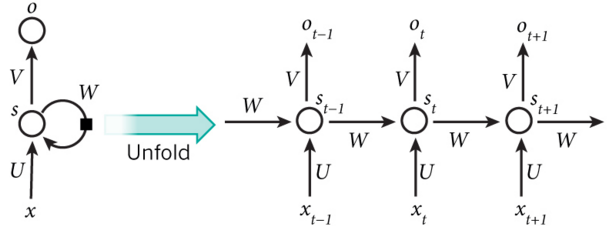
\includegraphics[width=\linewidth]{Images/rnn.PNG}
    \label{fig:rnn}
    \caption{Ontrolling van een recurrent neuraal netwerk}
\end{figure}

Het voorspellen van een zin met een RNN gebeurt woord per woord. Op basis van de eerder waargenomen woorden kan een softmax laag een kansverdeling maken voor het volgende woord. Met behulp van beam-search of het samplen van het meest waarschijnlijke woord, is het netwerk in staat om taal te genereren. Tijdens de trainingsfase worden woorden in de vorm van een vector aan het netwerk gegeven. Deze encodering kan gebruik maken van one-hot codering, ze kan random zijn, of er kan gebruik gemaakt worden van word embeddings zoals bijvoorbeeld \emph{word2vec}\cite{Mikolov2013}. Deze codering zelf kan ook deel uitmaken van het netwerk. Als dit het geval is, kan de codering verbeteren tijdens de training met behulp van terugpropagatie.

% CNN
\subsection{Convolutionele Neurale Netwerken}
Convolutionele Neurale Networken (ConvNets of CNN's) zijn een biologisch- ge\" inspireerde trainbare architectuur die invariante afbeeldingskarakteristieken kan leren. \cite{LeCun2010} Ze bieden een hi\"erarchische representatie van een afbeelding en zijn van nut in tal van visuele taken.\cite{Girshick2014}\cite{ciresan2012multi}\cite{lawrence1997face}
Een CNN is een 'Deep Learning' architectuur bestaande uit verschillende niveaus. De input en output van elk niveau is een verzameling van arrays die men een 'feature map' noemt. Op elke output is de feature map een representatie van een bepaald kenmerk van de afbeelding van alle mogelijke locaties van de input. Elk niveau bestaat standaard uit drie lagen: een filter bank laag, een non-linearity laag en een feature pooling laag. Na een aantal van deze niveaus is er nog een classificatielaag.
Trainen van dit netwerk kan gesuperviseerd met behulp van terugpropagatie, maar ook zeer snel ongesuperviseerd waardoor er geen nood is aan zeer grote gelabelde datasets. CNN's zijn in staat om veel sneller concepten te leren dan gewone feedforward netwerken, terwijl ze theoretisch slechts iets mindere resultaten kunnen bekomen. Een CNN gebruikt op elk niveau kleine rechthoekjes uit de vorige laag die bovendien mogen overlappen. Door deze overlapping is het netwerk translatie-invariant.

E\'en van de meest succesvolle toepassingen van CNN's is objectdetectie. Deze vooruitgang was vooral te wijten aan een paper\cite{Krizhevsky2012a} die CNN's gebruikt voor het oplossen van de ImageNet challenge.\cite{ILSVRC15}
Dit is een competitie waarin afbeeldingen moeten worden geclassificeerd in een aantal voorgedefini\"eerde categori\"en. De gebruikte architectuur bestaat uit 8 lagen waarvan 5 convolutioneel en 3 volledig verbonden. Ze gebruiken bovendien verschillende technieken om overfitting te vermijden. Als classificatielaag gebruiken ze softmax zodat het netwerk een kansverdeling over de verschillende categori\"een leert. De architectuur kan worden gezien in figuur \ref{fig:AlexNet} en  is een variant op de standaardarchitectuur die hierboven werd beschreven. Dit netwerk was het best presterende netwerk voor de wedstrijd in 2012. Ondertussen zijn nog diepere architecturen voorgesteld die op dezelfde en recentere wedstrijden nog betere resultaten bekomen. Het netwerk (VGGNet)\cite{Arge2015} dat wij gebruiken bestaat uit 16 lagen en is publiek beschikbaar met behulp van Caffe\cite{Jia2014}. De feature maps van verschillende outputlagen van dit netwerk dienen als input voor andere taken dan de ImageNet Challenge. Zo kan de output van de laatste laag voor de classificatielaag worden beschouwd als een representatievector voor de hele afbeelding. Output van andere lagen is een representatie voor lagere  afbeeldingskenmerken. 
\begin{figure}[tb]
	\centering
	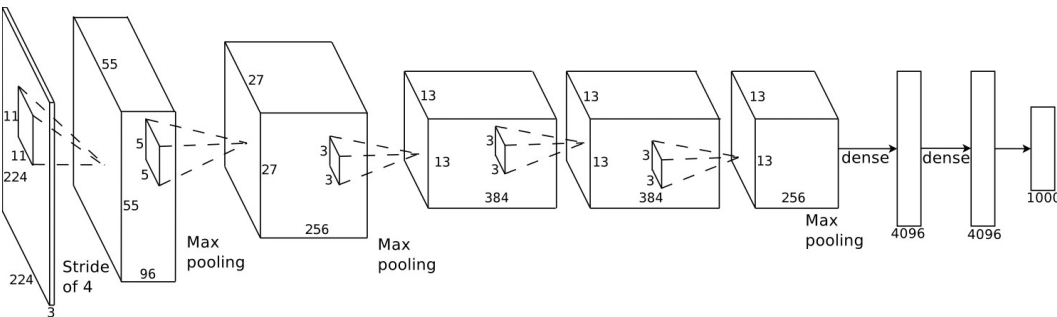
\includegraphics[width=\linewidth]{Images/cnn.PNG}
	\label{fig:AlexNet}
	\caption{Convolutioneel Neural Netwerk gebruikt door \cite{Krizhevsky2012a} voor classificatie van afbeeldingen}
\end{figure}


% LSTM
\subsection{Long Short Term Memory Neurale Netwerken}
Long Short Term Memory (LSTM) is een vorm van RNN die geheugencellen bevat. Door deze cellen is het netwerk in staat om op lange termijn informatie over de input bij te houden. Elk LSTM blok heeft een aantal gates om te bepalen of de input moet onthouden worden, en of een vorige waarde moet bijgehouden of vergeten worden. De output van de cellen is bijgevolg afhankelijk van alle eerder geobserveerde inputs. Op figuur \ref{fig:lstm} is te zien hoe een LSTM-blok er uitziet.\cite{Google}\cite{SeppHochreiter1997}

\begin{figure}[tb]
    \centering
    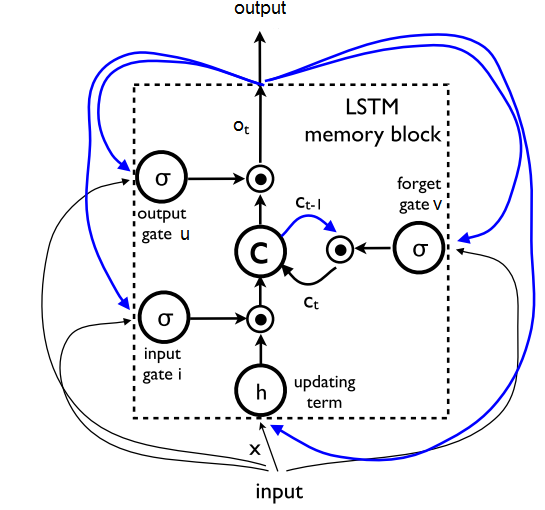
\includegraphics[width=\linewidth]{Images/lstm.PNG}
    \label{fig:lstm}
    \caption{Long Short Term Memory geheugenblok}
\end{figure}

LSTM netwerken worden net als RNN gebruikt als taalmodellen en zorgen over het algemeen voor hogere kwaliteit. Dit komt doordat LSTM netwerken over een langere periode dan een gewone RNN informatie kan onthouden. Hierdoor is het mogelijk om sequenties met events die gescheiden zijn door een langere periode, te modelleren. 

% LDA
\section{Latent Dirichlet Allocation}
Latent Dirichlet Allocation is een generatief probabilistisch model voor dsicrete data. Een van de meest gebruikte toepassingen hiervan is het modelleren van een een verdeling van onderwerpen in een set van tekstdocumenten. Dit conecpt is gebaseerd op de veronderstelling dat elk document een zeker kansverdeling heeft over alle mogelijke onderwerpen. Deze onderwerpen hebben dan een kansverdeling over alle mogelijke woorden. Zo kan de kans dat een bepaald document $d_j$ een bepaald woord $w_i$ bevat worden geschreven als een som over alle verschillende topics (formule \ref{formule:lda}). 

\begin{equation}
    \label{formule:lda}
    P(w_i | d_j) = \sum\limits_{k=0}^{n_{topics}}P(w_i|topic_k)P(topic_k|d_j)
\end{equation}

Het generatieve aspect van LDA is te zien in figuur \ref{fig:lda}. Op basis van twee Dirichlet priors $\alpha$ en $\beta$ word een kansverdeling over de onderwerpen gesampled per document ($\theta$), alsook een kansverdeling over de woorden voor elk onderwerp ($\phi$). Uit $\theta$ wordt voor elke positie $i$ in een document $j$ een onderwerp gesampled ($z_{ji}$). Het samplen van de woordverdeling voor dit onderwerp leidt tot het woord $w_{ji}$. Trainen van een LDA model gebeurt bijvoorbeeld met Gibbs sampling, en leidt tot de verdelingen $\theta$ en $\phi$.

\begin{figure}[tb]
    \centering
    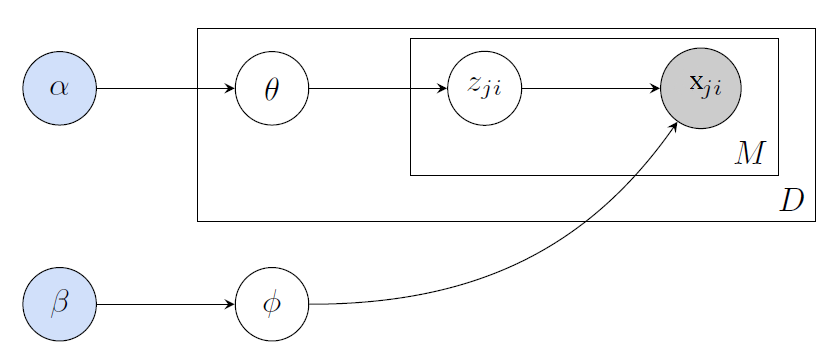
\includegraphics[width=\linewidth]{Images/lda.png}
    \label{fig:lda}
    \caption{Grafische weergave van LDA}
\end{figure}


%  Stacked CCA
\section{Stacked Canonical Correlation Analysis}
Canonical Correlation Analysis (CCA) is een methode die gebruikt wordt om een covariantiematrix van twee datasets te berekenen. Dit houdt in dat er een projectie wordt gemaakt naar een gemeenschappelijke ruimte voor beide datasets. In het onderzoek naar image captioning kan dit bijvoorbeeld leiden tot een multimodale mapping van afbeeldings- en beschrijvingsrepresentatie. 

Stacked CCA, gebaseerd op Stacked Auxiliary Embedding kan op basis van extra informatie een verbeterde mapping maken. Een voorbeeld hiervan is een dataset van ge-annoteerde foto's, versterkt met een dataset die per foto een set van stukjes van de foto met een aparte beschrijving. De representaties van de foto's en annotaties uit de dataset kunnen verbeterd worden door gebruik te maken van de informatie uit de extra dataset.

Om de uiteindelijke augmentatie te bereiken, zijn er een aantal stappen nodig. Uit de extra dataset volgt een eerste set van CCA projecties ($A$, $B$). Daarna volgt een projectie van de originele dataset ($X$, $Y$) naar de multimodale ruimte, door vermenigvuldiging met $A$ en $B$, resulterend in projecties $AX$ en $BY$. Vervolgens transformeren we $AX$ en $BY$ volgens de niet-lineaire functie $\phi(x)$. Concatenatie van de originele dataset met het resultaat van de niet-lineaire transformatie leidt tot $\hat{X} = [X, \phi(XA)], \hat{Y} = [Y, \phi(YB)]$. Een laatste stap in het proces is het berekenen van een LDA projectie die gebaseerd is op $\hat{X}$ en $\hat{Y}$, wat resulteert in $U$ en $V$.


Om de dimensionaliteit van de projectie te verhogen wordt voor $\phi(x)$ een random Fourier Feature (RFF) mapping gebruikt. Deze RFF is een functie gebaseerd op de gemiddelde afstand tot de vijftigste dichtste buur van de data. Voor elke foto en caption wordt gekeken welke andere foto of caption de vijftigste dichtste buur is, om vervolgens het gemiddelde te nemen van alle afstanden. De exacte berekening is $\phi(\mathbf{x})=\sqrt{2}cos(\mathbf{x}R+\mathbf{b})$. $R$ is een matrix die verkregen wordt door sampling van een normaalverdeling met gemiddelde 0, en standaardafwijking $\sigma^2$, waarbij $\sigma$ overeen komt met de eerder berekende gemiddelde afstand. Vector $b$ is resultaat van sampling uit een uniforme verdeling [0,1].

De projectie van een ongeziene afbeelding is het resultaat van het achtereenvolgens uitvoeren van alle transformaties. Voor vector $\mathbf{x}$ geeft dit $\mathbf{\hat{x}} = U[\mathbf{x}, \phi(A\mathbf{x})]$. Deze representatie kan gebruikt worden als een verbeterde versie van de originele image vector, bijvoorbeeld bij een image retrieval taak.